\chapter{Sprint zéro}\label{sprintzero}
Le sprint zéro n'est pas un sprint comme les autres, l'appellation de sprint peut être trompeuse. 
En effet, ce sprint ne donnera pas lieu à un incrément du logiciel, il n'y aura donc pas de revue de sprint. 

Cependant, cette phase est indispensable au bon fonctionnement du développement logiciel. 
Ainsi, lors de cette phase nous avons effectués plusieurs choses.

\section{Création de l'équipe de développement}
Notre équipe s'est formée assez rapidement, elle à surtout été créer par affinités. Mais également, 4 membres
de l'équipe ont effectués leurs projet de DUT ensemble, ainsi ils connaissaient déjà leurs façons de travailler.

L'équipe est ainsi composée de 6 membres : 
\begin{itemize}
	\item David \bsc{Bernard}
	\item Mathias \bsc{Faure}
	\item Antoine \bsc{Incorvaia}
	\item Lucas \bsc{Le gouic}
	\item Antoine de \bsc{Roquemaurel}
	\item Clément \bsc{Vannier}
\end{itemize}

\section{Choix des technologies utilisées}\label{choixTechno}
	\subsection{Développement}
		Une fois l'équipe composée, nous avons choisis la technologie avec laquelle nous allons développer le logiciel.
	 
		Nous avons donc passer en revues nos possibilités: 
		\paragraph{\texttt{Windev}} AGL\footnote{\textbf{A}telier de \textbf{G}énie \textbf{L}ogiciel} disponible sous Windows permettant de créer des logiciels
		assez rapidement. Cependant, la prise en main du logiciel est assez difficile, mais également, une fois effectué, la maintenance du logiciel
		est difficile. La rapidité d'exécution peut être discutable. 
		\paragraph{\texttt{Java} avec \texttt{Swing}} Java est un langage Orienté Objet multi-plateforme, lié à la bibliothèque \texttt{Swing} peut 
		permettre de créer des interfaces graphiques simples. Cependant, aucun de nous n'ayant d'expérience dans les bases de données
		en \texttt{Java}, nous risquions de perdre du temps à l'apprentissage.
		\paragraph{\texttt{C++} avec \texttt{Qt}} C++ Est un langage Orienté Objet, multi-plateforme, grâce à la bibliothèque \texttt{Qt} nous 
		pouvons créer une interface simple et ergonomique en se servant de l'EDI\footnote{Environnement de Développement Intégré} \texttt{QtCreator}. 
		Deux personnes de l'équipe ont de d'expérience dans les bases de données et les interfaces graphiques en \texttt{Qt}. Ainsi
		ils pourront aider les autres à se former. 

		Nous avons donc choisis d'utiliser le \texttt{C++} avec la bibliothèque \texttt{Qt}, elle nous permettra de créer un logiciel simplement,
		et d'avoir une base de données derrière.
	\subsection{Organisation}
		Afin de favoriser le développement via une méthode Scrum nous avons choisis d'utiliser une application de gestion de projet
		appelé \texttt{Redmine}. 
		Cette application était donc disponible à toute l'équipe via le web, cela nous permet de pouvoir tenir à jour le backlog produit, mais également
		de pouvoir assigner des tâches simplement. 
		Un tableau généré par Redmine de toutes nos tâches est disponible à l'annexe\ref{tableauTaches}page \pageref{tableauTaches}.
		\begin{figure}[H]
			\begin{center}
				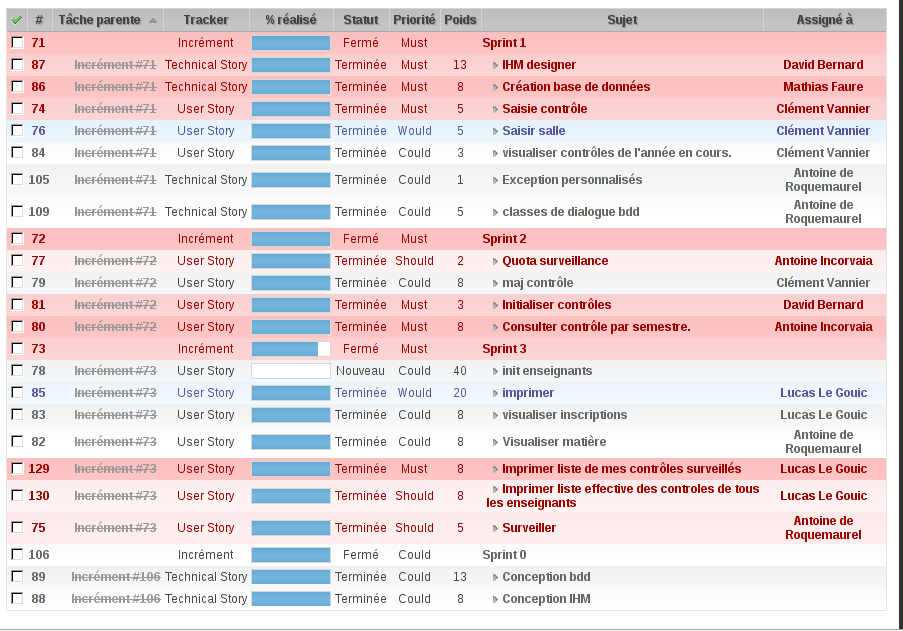
\includegraphics[width=17.5cm]{images/screenRedmine.png}
			\end{center}
			\caption{Capture d'écran des User et Technical stories dans Redmine}
		\end{figure}


\section{Planning poker}
	La technique du planning poker connait un succès grandissant auprès des équipe Scrum\footnote{En fait il ne s'agit pas de poker ni de planning, un nom plus approprié
	serait ``estimation de backlog''.}
	C'est une séance d'estimation en groupe, avec des cartes, qui combine le jugement d'expert et l'estimation par analogie.

	Ainsi, nous avons pus donner des poids aux différentes User Stories, mais nous avons également estimés les Technical stories.
	Les différents poids choisis sont disponibles en annexe \ref{tableauTaches} page \pageref{tableauTaches}.
\section{Conception}
	Une fois le planning poker effectué, nous avons effectué la conception du logiciel, étape extrêmement importante afin d'avoir un logiciel stable et facile à maintenir, cela nous à donc obliger à créer des 
technical stories

\subsection{Base de donnée}
	Nous avons donc conçut une base de donnée qui soit facile à utilisé et qui soit la plus performante possible. Ainsi, nous avons effectués un modèle de la base, mais également un jeu d'essai afin de pouvoir
effectuer des tests.

\subsection{Interface}
	Nous avons également conçut l'IHM\footnote{Interface Homme Machine} du logiciel, celle-ci devait être la plus ergonomique possible, pour avoir un logiciel facile à utiliser.

	L'interface Homme Machine du logiciel est disponible à l'annexe \ref{ihm} page \pageref{ihm}.	
